\documentclass[12pt, a4paper]{article}
\date{}
\usepackage{amsmath}
\usepackage{graphicx}
\begin{document}
\title{Equations différentielles utilisées}
\maketitle

\smallskip

\Large $t' = H_0*t \;,\; k=0 => \Omega_K=0$

$ a(t_0)=1 \;,\; t_0 = 0 = now$ 

\medskip

$da/dt' = \sqrt{\Omega_{\Lambda}*a^2+\Omega_{m0}/a+\Omega_{ro}/a^2}$
\\

UNIVERS $\Lambda$CDM
\\
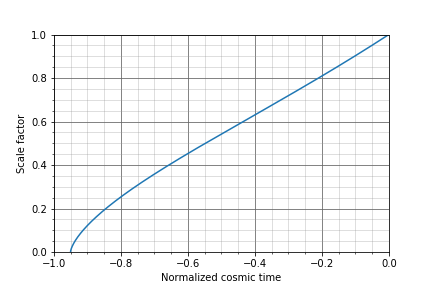
\includegraphics{Scale_factor}
\newpage

UNIVERS DE SITTER
\\
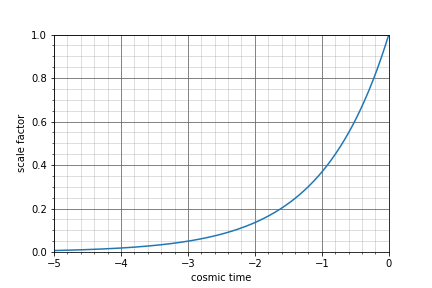
\includegraphics{DeSitter}

\newpage
UNIVERS EINSTEIN DE SITTER
\\
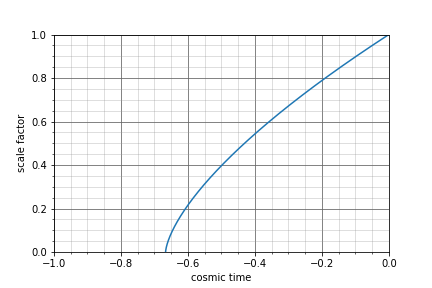
\includegraphics{EinsteinDeSitter}

\newpage
\bigskip

$dT_{bar}/dt' = -2 \frac{da}{dt'}\frac{1}{a} T_{bar}-\frac{8\sigma_Ta}{3m_ecH_0}\; T_{rad_0}^4 (T_{rad_0}/a-T_{bar})\frac{1}{a^4} \; x_e(T_I/T_{bar})$

\medskip

$T_I = 13.6ev/k_b$


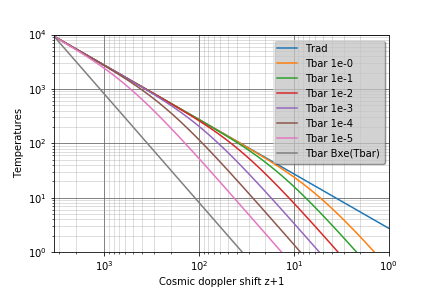
\includegraphics{Temperatures}

\newpage
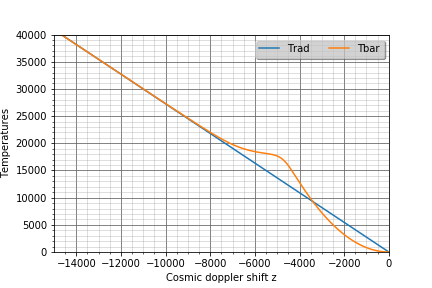
\includegraphics{TemperaturesL}

\newpage

$x_e(x)=1-erf(\sqrt{x})+2*\sqrt{x}*\exp(-x)/\sqrt{\pi}$


\includegraphics{XE}

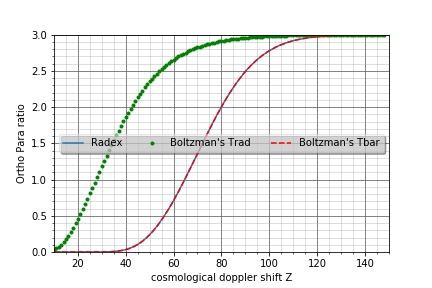
\includegraphics{rop}

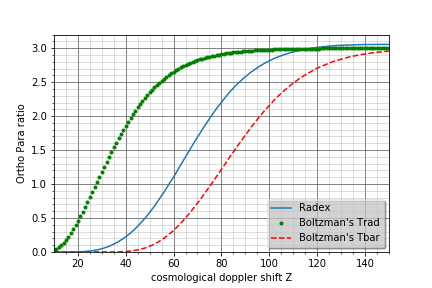
\includegraphics{rop2}

\end{document}